%%%%%%%%%%%%%%%%%%%%%%%%%%%%%%%%%%%%%%%%%%%%%%%%%%%%%%%%%%%%%%%%%%%%%%%%
\chapter{Background}
\label{ch:background}
%%%%%%%%%%%%%%%%%%%%%%%%%%%%%%%%%%%%%%%%%%%%%%%%%%%%%%%%%%%%%%%%%%%%%%%%

Machine Learning popularity exploded in last years. If you work in tech
it's hard you didn't heard about large public datasets, neural
networks, deep learning, or just how people speculates a majority of
jobs will be substitued by machine trained on our data.

Apart from a noisy hype, many services are actually built using Machine
Learning and they wouldn't be possible without it. Think of how Spotify
generates playlists that are perfectly tailored to you musical taste,
or how YouTube gives you perfect suggestions even when you should do
more serious work.

More and more developers are getting interested in this kind of
technology and as more people work on these topics more people build
better tools, empoweing larger majorities of developers to write
services using Machine Learning.

\section{Machine Learning}

Quoting
Wikipedia\footnote{https://en.wikipedia.org/wiki/Machine\_learning}

\begin{quote}
Machine learning is a field of computer science that uses statistical
techniques to give computer systems the ability to "learn" (e.g.,
progressively improve performance on a specific task) with data,
without being explicitly programmed.
\end{quote}

\begin{figure}
  \centering
  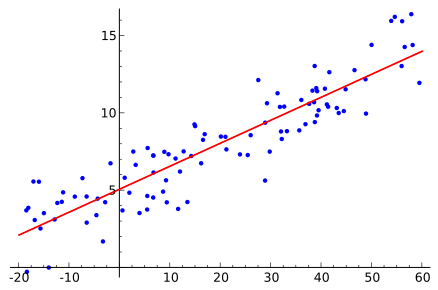
\includegraphics[width=0.5\linewidth]{wikipedia-linear-regression.png}
  \caption{A linear model built out of a dataset. By Sewaqu [Public
      domain], from Wikimedia Commons.}
\end{figure}

A typical example to introduce people with some scientific preparation
to this topic is the one of Linear
Regression\footnote{https://en.wikipedia.org/wiki/Linear\_regression}.
In linear regression you have data coming in pairs $(x, y)$ and you
think that $y$ can be linearly dependent on $x$. That is, your
hypothesis is that

\begin{equation}
  Y = w X + b
  \label{eq:linear-model}
\end{equation}

where $w$ and $b$ are called the weight and the bias
respectively\footnote{In other field, $w$ and $b$ are more commonly
  known as the slope and the intersept. In fact when data is expressed
  by two dimensions the model is easily visualizable as a line ---
  whose definition is the same as of Equation \ref{eq:linear-model}.}.

You don't know which are the \emph{correct} values for the weight and
the bias so you either estimate it using analytic methods like the ones
you probably learned in some math course or you derive the two values
using an iterative procedure that using the data minimizes the distance
between the data you have from the data you would compute using
Equation \ref{eq:linear-model} via current values for $w$ and $b$.

The function that computes the distance is generally called the
\emph{loss} function and can be as simple as the $L_1$
distance\footnote{https://en.wikipedia.org/wiki/Taxicab\_geometry\#Formal\_definition}
--- i.e. the difference of the two values. Instead the algorithm that
minimizes the loss can be any minimization procedure; one of the most
known one is called the gradient
descent\footnote{https://en.wikipedia.org/wiki/Gradient\_descent}.

The gradient descent procedure constists of iteratively computing

\begin{equation}
  \boldsymbol{x}_{n+1} = \boldsymbol{x}_n - \gamma
  \nabla{F}(\boldsymbol{x}_n)
\end{equation}

where $\gamma$ is the so-called \emph{learning rate} while
$\nabla{F}(\boldsymbol{x}_n)$ is the gradient of the loss function $F$
evaluated at $\boldsymbol{x}_n$. The idea behind the procedure is that
the gradient --- or the derivative, in the bi-dimensional case --- is
used to find the \emph{direction} in which the function is growing;
then it does an iterative step (how big depends on the
learning rate $\gamma$) in the \emph{opposite} direction. That is, the
procedure identifies where the loss functions is growing to perform a
step towards a minimum instead. The minimum is of course local --- it depends on
where the procedure starts --- and there's no guarantee that the
algorithm will succeed.

This algorithm has nothing to do specifically with linear regression. It's a general
minimization algorithm. In fact, later in the thesis we'll use it even
if we never touched the topic of linear regression again.

\section{Neural Networks}

\begin{figure}
  \centering
  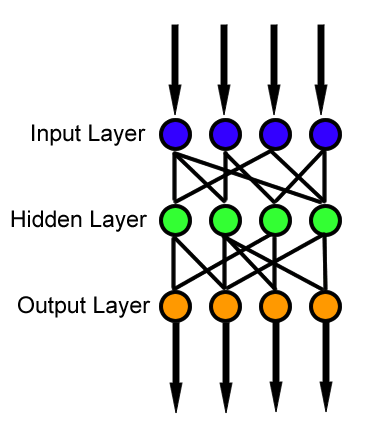
\includegraphics[width=0.5\linewidth]{wikipedia-neural-network.png}
  \caption{Neural network example. By User:Paskari [Public domain], via
    Wikimedia Commons}
  \label{fig:wikipedia-neural-network}
\end{figure}

A neural network is one of the many models studied in Machine Learning.
There are a variety of neural networks types, but the ones we used
throughout the thesis are called feedforward neural
networks\footnote{https://en.wikipedia.org/wiki/Feedforward\_neural\_network}.

A feedforward neural networks is perhaps the simplest possible neural
network and it is the one that most people are first exposed to. It
computes the composition of a linear function followed by the
application of a \emph{non}-linear function, called the activation
function.

Typically the linear function is

\[ XW + b \]

where X is a batch of inputs, while $W$ and $b$ are \emph{learned} by the
model.

The activation function can be a \emph{sigmoid-like} function such as
the softmax
\footnote{https://en.wikipedia.org/wiki/Softmax\_function} or the
simple
ReLU\footnote{https://en.wikipedia.org/wiki/Rectifier\_(neural\_networks)}
function

\begin{equation}
  \text{ReLU}(z) = \text{max}(0, z)
\end{equation}

This sequence of linear function and activation function can be 
\emph{repeated} multiple times increasing the hidden layers of neurons.
Having different numbers of hidden layers and of different width can
improve the performance of the model. When the network consists of
many layers, the network is referred to be a \emph{deep} neural
network. As a rule of thumb, the more the layers the better the performance
of the model. Yet, that's not always the case \emph{and} the deeper the
slower is to train that model.

In fact, deep learning is not a new idea and many considers the recent
interest in neural networks as a consequence of the current available
computational power that wasn't there in the 20th century.

\begin{quote}
  Advances in hardware enabled the renewed interest. In 2009, Nvidia
  was involved in what was called the ``big bang'' of deep learning, ``as
  deep-learning neural networks were trained with Nvidia graphics
  processing units (GPUs).'' That year, Google Brain used Nvidia GPUs to
  create capable DNNs. While there, Ng determined that GPUs could
  increase the speed of deep-learning systems by about 100 times. In
  particular, GPUs are well-suited for the matrix/vector math involved
  in machine learning. GPUs speed up training algorithms by orders of
  magnitude, reducing running times from weeks to days. Specialized
  hardware and algorithm optimizations can be used for efficient
  processing.\footnote{https://en.wikipedia.org/wiki/Deep\_learning\#History}
\end{quote}

The way we used neural networks has been for classification tasks, that
is given an input and a set of classes we want the network to be able
to assign that input to the correct class.

To understand how neural networks are used to perform classification it
is useful to know the concept of one-hot encoding of data. In one-hot
encoding

\begin{quote}
the legal combinations of values are only those with a single high (1)
bit and all the others low
(0).\footnote{https://en.wikipedia.org/wiki/One-hot}
\end{quote}

One-hot encoding is used to map classes (cat, dog, mockingbird, etc.)
in the training set to \emph{states} of the output neurons in the
neural network.

During the training phase the network is \emph{shown} a
configuration of the input neurons (the single input example) and a
configuration of the output neurons (the class of the input example
one-hot encoded), and the network is \emph{confronted} with the
configuration of the output it obtains using its current weights and biases
in the hidden layers and \emph{tries} to reduce this distance. Of
course, it's the gradient descent procedure that does this job, the
network is actually a \emph{passive} object.

\section{Adversarial examples}

Just like gradient descent is used to change the weights and biases of
the network to reduce the distance from the one-hot encoded class and
the actual output of the network, we can use gradient descent on the
input data to reduce the distance from the current output of the network to
another output of our choice. This way we can manipulate classification.

What we get is an input data generated from the original input but
slightly modified in such a way that the input is \emph{misclassified}.
These generated inputs are called \emph{adversarial examples}.

\begin{figure}
  \centering
  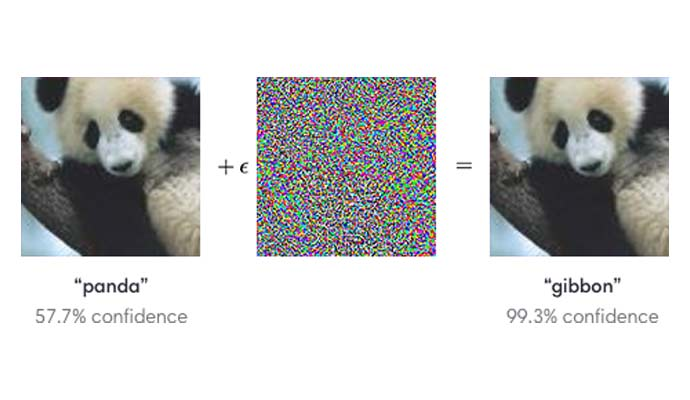
\includegraphics[width=\linewidth]{panda-gibbon.jpg}
  \caption{Panda misclassified to a gibbon, using carefully crafted
    noise.}
\end{figure}

There are different techniques to generate these adversarial examples.
One of the most notable one is called fast gradient sign and has been
introduced by Goodfellow, et al. in \cite{goodfellow6572explaining}.
There's no need to know much about this attack, as many libraries
already implements this technique. In fact we used that \emph{as a service}
without caring too much of the details.

\section{...}

%% Any cited url has been scanned and archived using the Wayback Machine
%% as of October 2018.
